\documentclass[10pt]{article}
\usepackage[margin=0.82in]{geometry}
\usepackage[T1]{fontenc}
\usepackage{lmodern,booktabs,tabularx,graphicx,xcolor,amsmath,microtype,hyperref}
\hypersetup{colorlinks=true,linkcolor=blue,urlcolor=blue}
\setlength{\parskip}{5pt}
\setlength{\parindent}{0pt}
\newcommand{\source[1]}{\texttt{#1}}
\begin{document}
\begin{center}
{\LARGE\bfseries Intent2Proof: AXI-Lite Abstraction Qualification}\par
\vspace{4pt}{\large Source-Grounded Refinement Probe and Pinned RTL Benchmark}\par
\vspace{3pt}\textit{Supplementary preliminary experiment; proof status explicitly separated}\par
\end{center}
\section*{Research question and result}
The previous heterogeneous AXI-Lite experiment separately proved selected control properties on a real open-source AXI-Lite interconnect and a smaller candidate contract bridge. However, independent safety proofs are not a certificate that the bridge preserves the concrete implementation's behaviors. We test a stricter, \emph{cycle-accurate observational relation} for accepted AXI read addresses under matched inputs.

\textbf{Observed local result.} The pinned upstream source drives \texttt{s\_axil\_arready} from a register initialized to zero. The candidate bridge drives \texttt{s\_arready} combinationally when idle and an address is presented. A source-anchored one-step Z3 model finds a handshake mismatch immediately after reset for both a single requester and two simultaneous requesters. A no-request control finds no mismatch. \textbf{These are limited source-to-equation checks, not full elaborated RTL equivalence proofs.}

\begin{center}\small
\begin{tabular}{@{}lccc@{}}\toprule
Post-reset situation & Upstream accept & Contract accept & Mismatch query\\\midrule
No read request & \texttt{00} & \texttt{00} & UNSAT\\
Master 0 read request & \texttt{00} & \texttt{01} & SAT\\
Both masters read request & \texttt{00} & \texttt{01} & SAT\\\bottomrule
\end{tabular}\end{center}

\begin{figure}[ht]\centering
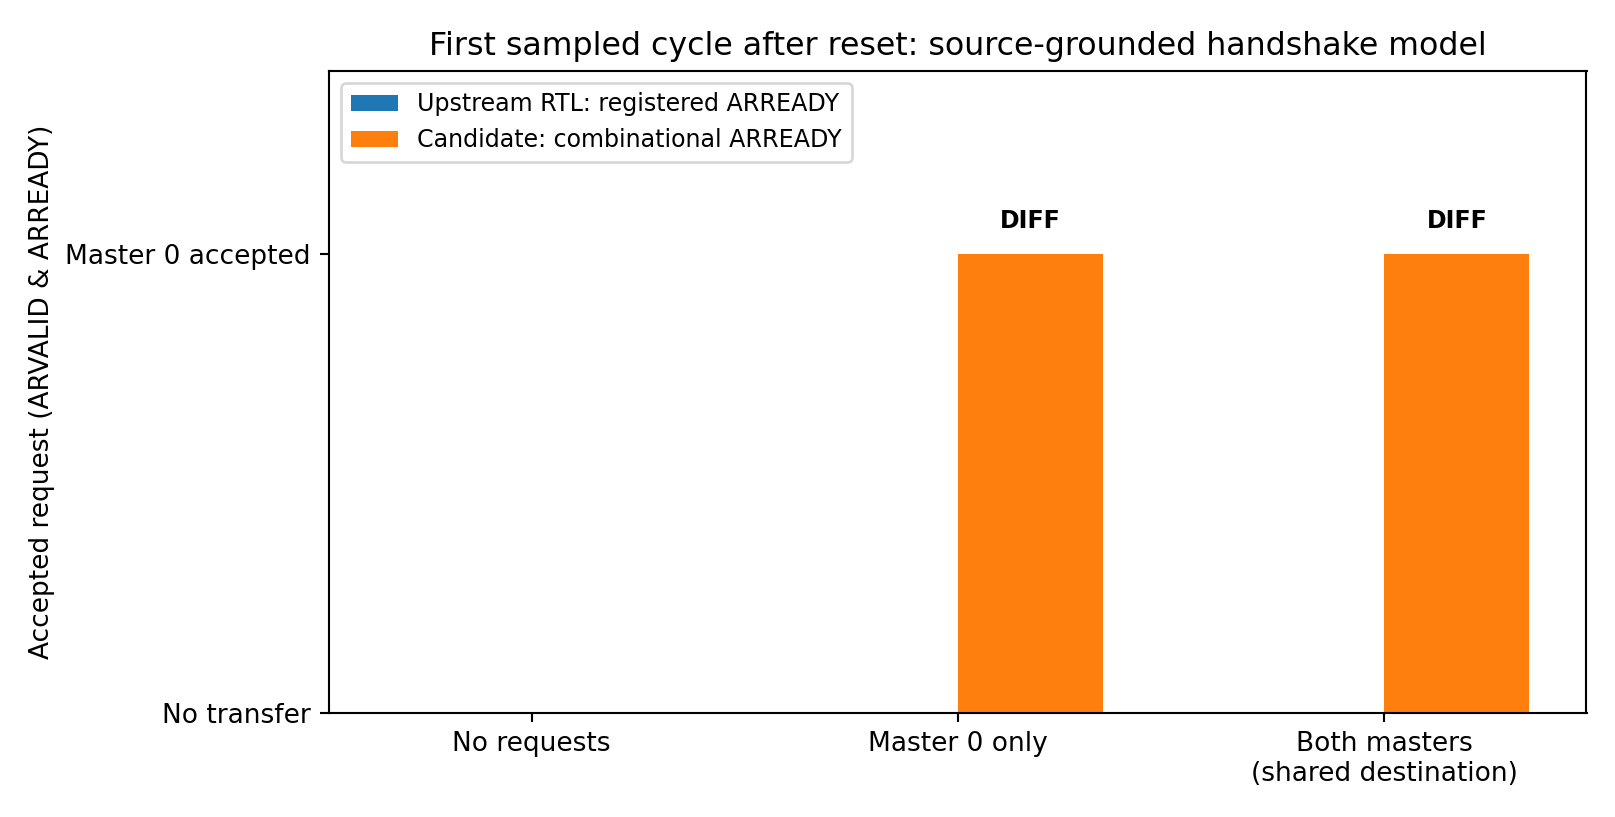
\includegraphics[width=.76\linewidth]{figures/figure1_handshake_difference.png}
\caption{Source-grounded first-cycle request-acceptance mismatch. This is not a completed full-RTL miter result.}
\end{figure}

\section*{Prepared real-RTL qualification and contention test}
The package bundles the original three upstream Verilog modules from commit \texttt{516bd5da...} (full SHA-1 in the manifest); their SHA-256 hashes are checked on every run. The previously identified 2-bit versus 4-bit response-bus width mismatch in the local integration is corrected.

Eight SymbiYosys tasks have been generated. Four test matched-input cycle-accurate read-acceptance equivalence and its negative/sanity coverage, one covers simultaneous same-destination requests followed by acceptance and completion for \emph{both} masters, one checks unbounded system safety under that destination policy, and two inject response-routing and shutdown errors.

The two-implementation miter compares the observed read-address transfer events, \(ARVALID\land ARREADY\). It also retains separate read-response observations for later extensions. Only the exact accepted-event relation is asserted in the first experiment. A mismatching witness refutes \emph{lockstep equivalence under the tested assumptions}; more permissive nondeterministic trace inclusion or stutter-tolerant refinement requires separate proof obligations.

\begin{figure}[ht]\centering
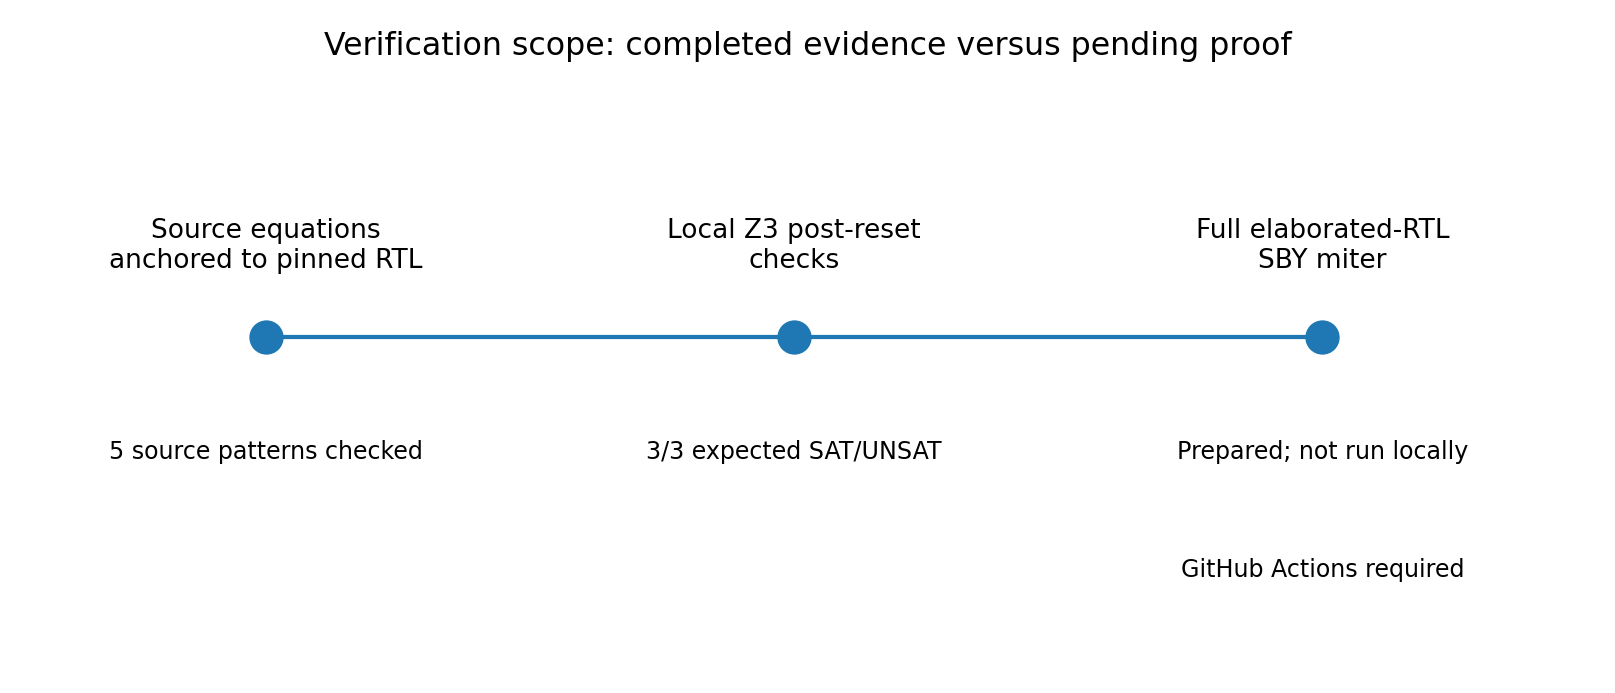
\includegraphics[width=.9\linewidth]{figures/figure2_evidence_boundary.png}
\caption{Separation of evidence executed in this container from the prepared GitHub formal tasks.}
\end{figure}

\section*{Execution scope and decision}
All \textbf{10 offline harness tests passed}; the local SMT checks returned their three expected SAT/UNSAT outcomes. The attempt to run the full-RTL formal tasks locally was correctly marked \texttt{BLOCKED\_MISSING\_FORMAL\_TOOLS}. \textbf{No new upstream SBY results, proof-time speedups, or automatic refinement certificates are claimed.}

Run the bundled root-level GitHub workflow \texttt{.github/workflows/intent2proof-axi-refinement.yml} and download \texttt{intent2proof-axi-refinement-evidence}. The formal result gate refuses automatic approval: even when an expected mismatch is demonstrated, the contract must be reported as \texttt{REJECTED} for cycle equivalence and \texttt{NOT\_PROVED} for general trace inclusion.

\textbf{Implication for the proposal.} This experiment tests the missing soundness obligation rather than just another isolated safety property. An abstract bridge can reduce AIG size and independently prove useful properties while failing to preserve the concrete bus's handshake timing. A revised contract must model the relevant registered-ready/arbitration behavior or establish an appropriate conservative relation before claimed solver reductions qualify as sound acceleration.
\end{document}
